
\section{Análisis de control con deflexión de flaps}

La torsión geométrica obtenida en la sección \ref{sec:ajuste_torsion} para lograr $C_{M_\text{cg}} = 0$ solamente es válida en la condición de diseño. En otras condiciones de vuelo será necesaria la deflexión de flaps/alerones para conseguir $C_{M_\text{cg}} = 0$. En esta sección se obtienen las relaciones $C_{M_\text{cg}} = f \left( C_L \right)$ para diversas deflexiones de flaps $\left( \delta_e \right)$. Posteriormente se determinan las deflexiones requeridas para obtener $C_{M_\text{cg}} = 0$ en dos condiciones de vuelo en planeo.

Según \cite{performace_hoIV} el Horten IV dispone de tres superficies de control, representadas en su figura 6. De izquierda a derecha son alerones, \emph{dive brakes} y \emph{drag rudders}. Se considera que para el control pueden utilizarse alerones y \emph{dive brakes}. Por consiguiente, los flaps se sitúan entre $3.75 \ \meter$ y $7.75 \ \meter$, \ie, $0.375$ y $0.775$ adimensionalizando con la envergadura. La relación cuerda flap -- cuerda ala se calcula usando las cuerdas medias aerodinámicas de ambos. Usando el método geométrico seguido en \ref{sec:ajuste_flecha}, para el flap $\overline{\overline{c}} = 0.2522 \ \meter$, con la que se obtiene una relación de $0.2314$. El factor de eficiencia del flap es el correspondiente a flap plano, \ie, $\eta = 0.8$.

Para obtener $C_{M_\text{cg}} = f \left( C_L \right)$ se simula el ala volante con deflexiones de flaps entre $-20\degrees$ y $20\degrees$ en incrementos de $5\degrees$, para ángulos de ataque de $-2 \degrees$, $4 \degrees$ y $10 \degrees$. Aplicando el procedimiento seguido en \ref{sec:ajuste_torsion}, se calcula $C_{M_\text{cg}}$ para tres $C_L$. Por último se calcula la regresión lineal de los puntos.

Las condiciones impuestas en el vuelo de planeo son máximo alcance y velocidad de descenso mínima. Para máximo alcance se requiere eficiencia aerodinámica máxima \cite{franchini}. Con la curva polar \eqref{eq:curva_polar_ala}, 
\begin{equation}
    C_{L_\text{max range}} = \sqrt{\frac{C_{D0}}{k}} = 0.5132
\end{equation}
Para mínima velocidad de descenso, \ie, máxima autonomía
\begin{equation}
    C_{L_\text{min speed}} = \sqrt{\frac{3 C_{D0}}{k}} = 0.8888
\end{equation}

En la figura \ref{fig:cmcg_flap} se representa el coeficiente de momentos CG en función del coeficiente de sustentación para las deflexiones de flap analizadas, así como los $C_L$ de las dos condiciones de vuelo de planeo estudiadas.
\begin{figure}[h]
    \centering
    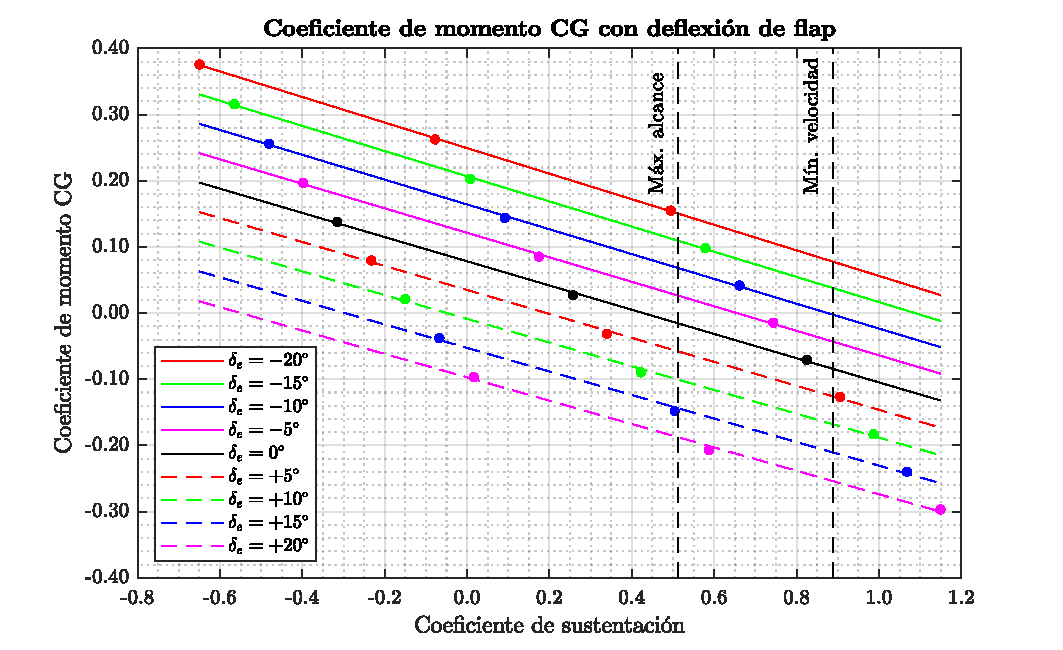
\includegraphics[width=\linewidth]{imagenes/control_flaps/cmcg_flap.pdf}
    \caption{Coeficiente de momento CG $( C_{M_{\text{cg}}} )$ en función del coeficiente de sustentación $\left( C_L \right)$ para deflexiones de flap $\left( \delta_e \right)$ entre $-20\degrees$ y $20\degrees$ y $C_L$ para condición de máximo alcance y mínima velocidad de descenso.}
    \label{fig:cmcg_flap}
    \vspace{-4mm}
\end{figure}

\noindent
Para un mismo $C_L$, a medida que crece $\delta_e$, $C_{M_\text{cg}}$ disminuye. Esto se debe al aumento en la curvatura del perfil, que provoca un incremento en la sustentación y a su vez un incremento en el momento generado.

De la figura \ref{fig:cmcg_flap} se aprecia que para lograr $C_{M_{\text{cg}}}$ en la condición de máximo alcance, es necesaria una deflexión de flap entre $-5\degrees$ y $0\degrees$. Por lo tnat de $-2.5\degrees$. En la condición de mínima velocidad de descenso, la deflexión de flap necesaria es de $-10\degrees$.

